\title{\bf Lecture 6 - Flaws\\}
\author{\bf Rylan Schaeffer and Vincent Yang\\}
\date{\bf \today \\}

\documentclass{article}
\renewcommand{\thesubsection}{\thesection.\alph{subsection}}
\usepackage{enumerate}
\usepackage{amsmath}
\usepackage{url}
\usepackage{graphicx}
\setlength{\oddsidemargin}{0in}
\setlength{\evensidemargin}{0in}
\setlength{\textheight}{9in}
\setlength{\textwidth}{6.5in}
\setlength{\topmargin}{-0.5in}

\begin{document}
\maketitle

Note: This lecture is based on Princeton University's BTC-Tech: Bitcoin and Cryptocurrency Technologies Spring 2015 course.


\section*{Blockchain Applications}
\begin{itemize}
  \item What it can do:
    \subitem Have a large number of nodes with up-to-date information.
    \subitem Account for dishonest nodes
    \subitem Determine with non-negligible certainty the existance of an operation
    \subitem High cost of rewriting history
    \subitem Solution for conflicting information
  \item Smart Contracts
  \item NameCoin - DNS Server
  \item Colored coin - just link something physical to each digital coin
  \item Decentralized P2P Energy Networks, P2P Communication, P2P Logistics, etc.
  \item Deloitte created MVP - warranty bot that lets users send an image of a specially designed receipt via FB Messenger.
    \subitem Then, Deloitte's product can 'unwrap' a QR code and store the information on a blockchain.
    \subitem Gives proof of ownership, can be transferred, and proof it existed.
  \item Trading Ownership in an Online Marketplace - creators as well
    \subitem Blockai uses blockchain to help artists protect intellectual property
  \item File Storage
  \item HyperLedger - Linux Foundation
    \subitem Business Networks - anything of value can be tracked and traded.
    \subitem Manage flow of goods (supply chain), and related payments/share production logs.
    \subitem Fluent - just supply chain
  \item Tierion - verifiable record of any data/business process in block chain
    \subitem Use case example: Insurance - collect claims data and issue a blockchain receipt. Gives verifiable
    record of the time and content of initial claim - reducing errors, fraud, and cost of auditing claims.
  \item Similar to Tierion - Everledger (With Barclays) working on creating reliable receipts for luxury goods.
    \subitem Diamonds - If you have a 5 carat diamond, then serial number + 4 C's (Carat Weight, Cut, Color, Clarity) +
    angels + pavilions... ultimately 40 metadata points.
  \item Edgelogic: Blockchain with Internet of Things
    \subitem Example: sensor reports when something starts to go wrong that is covered by insurance, and automatically makes transfer
    that can be logged and referred to (binding) from insurer to claimant's account, without even the person knowing. 
  \item In summary:
\end{itemize}
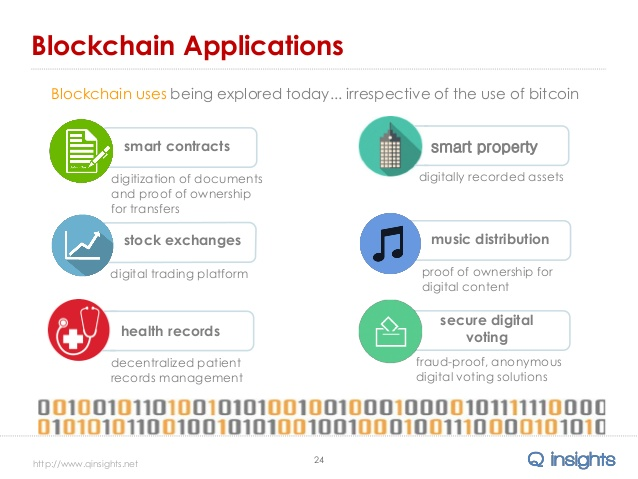
\includegraphics[height=4in]{alternative-payments-evolution-or-revolution.jpg}\\
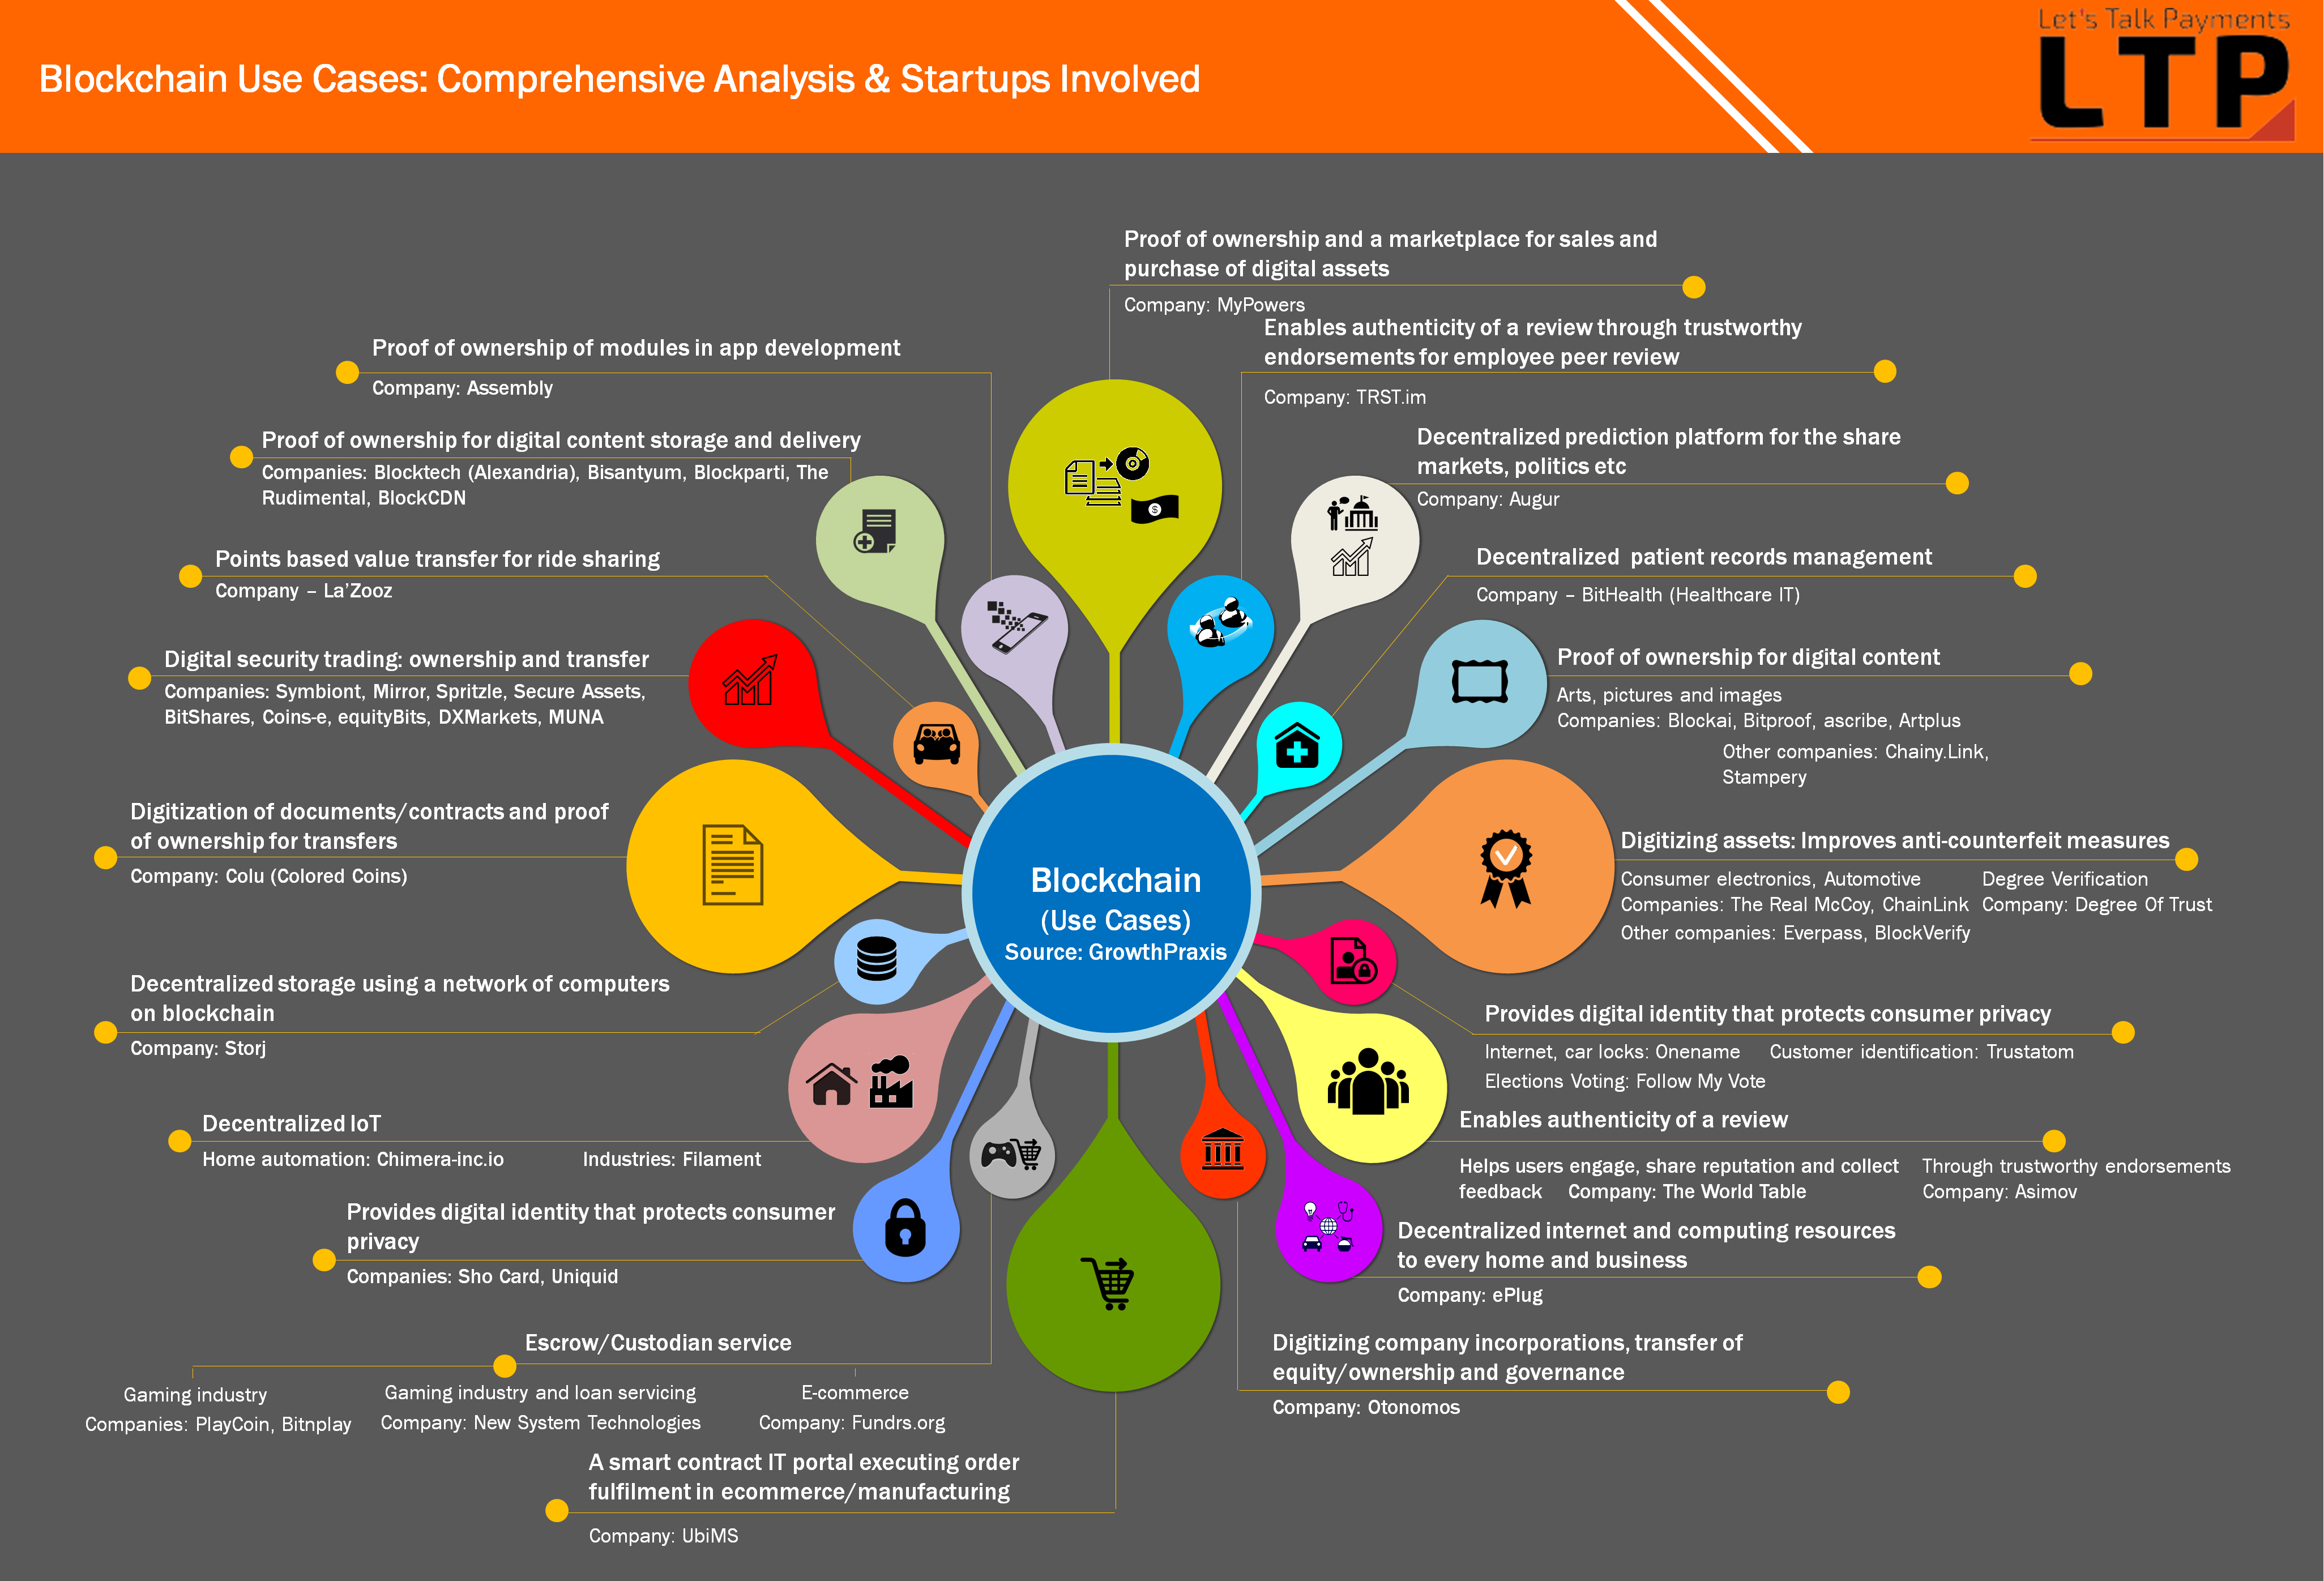
\includegraphics[width=\linewidth]{Blockchain-Usecases-and-Startups.png}

\section*{Project Planning}
\begin{itemize}
  \item Planning out your project is extremely important. 
  \item Understand the overall goal of the program, as well as key functions for how 
    each part comes together.
  \item Submit a plan by the end of the class. This plan should incorporate 
    \begin{enumerate}
      \item Each main component, as well as how you intend on completing it. 
      \item This plan should also incorporate a brief description of each component, and a general idea of how it works. 
        \subitem e.g. We want to create a mining based app, where people can only submit messages after completing proof of work. Two important components
        are the hash function and digital signatures. Cryptographic hash functions with signatures can be implemented with the Python rsa library.
        \subitem e.g. We want to create a rudimentary Cryptocurrency. MIT has a skeleton for this in java that we can pull from. Essential components are the BlockChain (universal ledger), 
      Signatures, Hashing.
      \item Lastly, the plan should incorporate a two week projection of goals - where you expect to be in two weeks, with respect to the whitepaper and implementation, as well as
        who is working on what.
    \end{enumerate}
    \item Checkpoint 2 - this submitted paper. 
      \subitem Feel free to ask Rylan and I for help and feedback during this time. 
\end{itemize}


\end{document}
